\chapter{ Аналитический раздел}
\label{cha:analysis}
\section{Постановка задачи}
В соответствии с техническим заданием в области компьютерной графики, необходимо реализовать программный продукт, предоставляющий визуализацию маятника Ньютона. Нужно определиться с выбором метода решения. Пользователь должен иметь возможность запуска и останова визуализируемой механической системы. В данной системе будут отсутствовать противодействующие силы, поэтому она будет действовать до тех пор, пока что пользователь не решит ее остановить. Полученное изображение должно четко показывать работу механической системы.

\section {Описание предметной области}
\textit{Компьютерная графика } -- занимает большой раздел в IT сфере. Она помогает решать многие задачи, актуальные в нашем времени. В компьютерной графике рассматривают обязательной задачей разработку алгоритмов визуализации трехмерных объектов \cite{bib2}. К примеру, визуализацию механических систем для демонстрации какого-то существующего явления без нужных, для данного явления, аппаратов.

\section {Описание алгоритмов}

\subsection {Некоторые теоретические сведения}

Прежде чем описывать алгоритмы, я хотела бы дать некоторые определения, чтобы читателю было проще воспринимать рассказанные ниже алгоритмы \cite{bib2,bib6}.

Алгоритмы удаления невидимых линий и поверхностей служат для определения линий ребер, поверхностей, которые видимы или невидимы для наблюдателя, находящегося в заданной точке пространства.

Решать задачу можно в пространстве:
\begin{enumerate}
	\item Объектном - мировая системе координат, высокая точность. Обобщённый подход, основанный на анализе пространства объектов, предполагает попарное сравнение положения всех объектов по отношению к наблюдателю.
	\item Изображений - в экранных координатах, системе координат, связанной с тем устройством в котором мы отображаем результат отображения (Графический дисплей).
\end{enumerate}

Под экранированием подразумевается загораживание одного объекта другим.

Под глубиной подразумевается значение координаты Z.

\subsection{Алгоритм Робертса}

Алгоритм Робертса -- решает задачу удаления невидимых линий. Работает в объектном пространстве. Он строго работает с выпуклыми телами. Если тело изначально является не выпуклым, то нужно его разбить на выпуклые составляющие. Алгоритм целиком основам на математических предпосылках, которые просты, точны и мощны \cite{bib1}.

Основные этапы:
\begin{enumerate}
	\item Подготовка исходных данных.
	\item Удаление линий, экранируемых самим телом.
	\item Удаление линий, экранируемых другими телами.
	\item Удаление линий пересечения тел, экранируемых самими телами, связанными отношением протыкания и другими телами.
\end{enumerate}

0. Подготовка исходных данных:

Для каждого тела сцены необходимо сформировать матрицу тела. Обозначают: V. Размерность: 4*n, где n - количество граней. Каждый столбец матрицы - это коэффициенты уравнения плоскости (4 коэффициента), проходящей через очередную грань тела.

Уравнение плоскости:

\begin{equation}
	Ax + By + Cz + D = 0
\end{equation}

В матричной форме выглядит следующим образом:

\begin{equation}
	[x\;y\;z\;1][P] = 0
\end{equation}

где 

\begin{equation}
	P = \left(
	\begin{array}{c}
			A \\
			B \\
			C \\
			D \\
		\end{array}
	\right)
\end{equation}

Тогда матрица тела будет выглядеть следующим образом:

\begin{equation}
	V = \left(
	\begin{array}{cccc}
			A_{1} & A_{2} & \ldots & A_{n} \\
			B_{1} & B_{2} & \ldots & B_{n} \\
			C_{1} & C_{2} & \ldots & C_{n} \\
			D_{1} & D_{2} & \ldots & D_{n}
		\end{array}
	\right)
\end{equation}

где n - количество граней.

Формирование матрицы:

Нужно найти коэффициенты каждой плоскости, проходящей через каждую грань тела. Располагая информацией о координатах 3 неколлинеарных точках, принадлежащий плоскости, можно найти коэффициенты данной плоскости. Плоскость однозначно задается 3 точками. Делим уравнение на d, при этом свободный член будет равен единице.

\begin{equation}
	{\begin{cases} 
			Ax_1 + By_1 + Cz_1 = -1 \\
			Ax_2 + By_2 + Cz_2 = -1 \\
			Ax_3 + By_3 + Cz_3 = -1 \\
		\end{cases}}
\end{equation}

Запишем в матричной форме:

\begin{equation}
	[X][C] = [D]
	\label{eq:ref1}
\end{equation}

где

\begin{equation}
	X = \left(
	\begin{array}{cccc}
			x_{1} & y_{1} & z_{1} \\
			x_{2} & y_{2} & z_{2} \\
			x_{3} & y_{3} & z_{3} \\
		\end{array}
	\right)
\end{equation}

~

\begin{equation}
	СC = \left(
	\begin{array}{c}
			A \\
			B \\
			C \\
		\end{array}
	\right)
\end{equation}

~

\begin{equation}
	D = \left(
	\begin{array}{c}
			-1 \\
			-1 \\
			-1 \\
		\end{array}
	\right)
\end{equation}

Решая уравнение (\ref{eq:ref1}), получаем значения коэффициентов уравнения плоскости: 

\begin{equation}
	[C] = [X]^{-1}[D]	
\end{equation}

Сформировав матрицу тела нужно проверить ее на корректность. 

Корректная матрица тела - это такая матрица, у которой любая точка, расположенная внутри тела, должна располагаться по положительную сторону от каждой грани тела. Т.е. при подставки координат любой точки, расположенной внутри тела в каждое из уравнение плоскостей в результате должно получаться положительное число. Если для очередной грани это условие не выполняется, то соответствующий столбец матрицы нужно умножить на -1. Чтобы не ошибиться с выбором точки, расположенной внутри матрицы тела, можно усреднить координаты всех вершин тела, либо взять полусумму координат максимальных и минимальных значений.

1. Удаление линий, экранируемых самим телом.

Для решения этой задачи нужно указать место расположения наблюдателя и направление его взгляда.

\begin{equation}
	E = |00-10|
	\label{eq:ref2}
\end{equation}

С одной стороны (\ref{eq:ref2}) это вектор взгляда наблюдателя, с другой стороны это вектор однородных координат точки, расположенной в минус бесконечности по оси z.

Для определения невидимых граней следует вектор взгляда E умножим матрицу тела V. Отрицательные компоненты полученного вектора будут соответствовать невидимым граням.

2. Удаление линий, экранируемых другими телами.

Наблюдатель находится в плюс бесконечности на оси z. Если на 1 этапе мы использовали вектор взгляда, то на 2 этапе мы используем координаты точки, в которой находится наблюдатель, обозначим как (\ref{eq:ref3}).

\begin{equation}
	g = |0010|
	\label{eq:ref3}
\end{equation}

Для определения невидимых точек ребра нужно построить луч, соединяющий точку наблюдения с точкой находящейся на ребре.
Точка будет невидимой, если луч на своем пути встречает в качестве преграды рассматриваемое тело.
Если тело является преградой, то луч должен пройти через тело.
Если луч проходит через тело, то он находится по положительную сторону от каждой грани тела.

3. Удаление линий пересечения тел, экранируемых самими телами, связанными отношением протыкания и другими телами.

Если тела связаны отношением взаимного протыкания, то образуются новые ребра, соответствующие линиям пересчения тел. Необходимо найти новые реба. Новые ребра можно получить путем соединения точек протыкания между собой. Вновь полученные ребра надо проверить на экранирование самими телами, связанными отношением протыкания. Оставшиеся видимые части ребер надо проверить на экранирование другими телами сцены.

Фактически на 3 этапе мы повторяем первые два этапа для новых ребер, которые получаются в результате протыкания тел.

~

Алгоритм Робертса хорошо применим для изображения множества выпуклых многогранников. Однако имеются недостатки: для визуализации более естественного изображения нам нужно уметь работать с тенью. В этом заключается один из недостатков. Без модификации и привлечения сторонних методов данный алгоритм не позволяет нам реализовывать тень. Также невозможно передать зеркальный эффект и преломление света.

\subsection{Алгоритм Варнока}

Алгоритм Варнока -- противоположен алгоритму Робертса. Решает задачу в пространстве изображений. Изображает видимые элементы. Единой версии алгоритма Варнока не существует. Можно рассматривать простейшую версию и более сложные версии алгоритма Варнока.

\begin{figure}[ht!]
	\centering{
		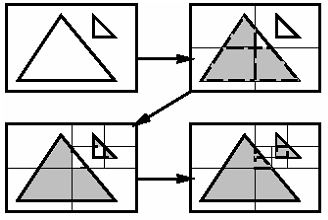
\includegraphics[width=0.5\textwidth]{img/warnock_algorithm_example2.png}
		\caption{Пример разбиения Алгоритмом Варнока}}
\end{figure}

Основная идея состоит в том, что необходимо найти ответ на вопрос о том, что изображать в очередном окне. Сначала окно имеет размеры экрана. Если мы точно не можем дать ответ, то мы окно делим на части (каждую сторону окна делим на две части). Вместо одного окна получаем 4 меньших размеров. Если снова не можем дать ответ, то продолжаем делить каждое окно на 4 части, пока не сможем дать ответ или окно не станет равным в 1 пиксель.

В простейшей версии алгоритма окно делится на подокна всякий раз, если это окно не пусто. Пределом деления является получения окна размером в 1 пиксель. Для одной точки легко определить ближайший к наблюдателю многоугольник (для этого нужно найти глубину каждого многоугольника в этой точки). В более сложных версиях делается попытка решения задачи для окон большего размера (больше одного пикселя). Для этого нужно провести классификацию многоугольников, рассматриваемых в алгоритме Варнока и действия, которые нужно предпринять в том или ином случае.

Классификация многоугольников:

\begin{enumerate}
	\item С окном связан один охватывающий многоугольник -- окно нужно закрасить цветом охватывающего многоугольника.  Рисунок \ref{fig:ref}a;
	\item С окном связан один пересекающий многоугольник -- выполняем отсечение многоугольника по границам окна и получаем один внутренний многоугольник. То есть сводим задачу к случаю с одним внутренним многоугольником.  Рисунок \ref{fig:ref}b;
	\item С окном связан один внутренний многоугольник -- окно нужно закрасить фоновым цветом, а затем выполнить растровую развертку единственного многоугольника. Рисунок \ref{fig:ref}c;
	\item Все многоугольники являются внешними по отношению к окну -- окно закрасить цветом фона.  Рисунок \ref{fig:ref}d;
\end{enumerate}

\begin{figure}[ht!]
	\centering{
		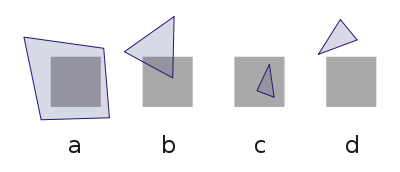
\includegraphics[width=0.6\textwidth]{img/warnock_algorithm_types.png}
		\caption{Классификация многоугольников в Алгоритме Варнока}
		\label{fig:ref}}
\end{figure}

К недостаткам алгоритма также можно отнести невозможность передачи зеркальных эффектов и преломления света. Также при визуализации сложной сцены число разбиений может стать очень большим, что приведет к ухудшению скорости.

\subsection{Алгоритм Вейлера-Азертона}

Алгоритм Вейлера-Азертона -- пытается минимизировать количество разбиений в алгоритме представленном выше (Алгоритме Варнока) путем разбиения окна вдоль границ многоугольника. Основой служит алгоритм Вейлера-Азертона, который используется для отсечения многоугольников.

Если многоугольники пересекают друг друга, то надо разбить один из них на два линей пересечения плоскостей присущих этим многоугольникам \cite{bib3}.

К недостаткам алгоритма относится сложность реализации, а также невозможность передачи зеркальных эффектов и преломления света.

\subsection{Алгоритм Z-буфера}

Алгоритм Z-буфера -- решает задачу в пространстве изображений. Сцены могут быть произвольной сложности, а поскольку размеры изображения ограничены размером экрана дисплея, то трудоемкость алгоритма зависит линейно от числа рассматриваемых поверхностей. Элементы сцены заносятся в буфер кадра в произвольном порядке, поэтому в данном алгоритме не тратится время на выполнение сортировок.

Буфер кадра (регенерации) - используется для заполнения атрибутов (интенсивности) каждого пикселя в пространстве изображения. Для него требуется буфер регенерации, в котором запоминаются значения яркости, а также Z-буфер (буфер глубины), куда можно помещать информацию о координате z для каждого пикселя.

Для начала нам нужно подготовить буферы. Для этого в Z-буфер заносятся максимально возможные значения z, а буфер кадра заполняется значениями пикселя, который описывает фон. Также нам нужно каждый многоугольник преобразовать в растровую форму и записать в буфер кадра. Сам процесс работы заключается в сравнении глубины каждого нового пикселя, который нужно занести в буфер кадра, с глубиной того пикселя, который уже занесён в Z-буфер. В зависимости от сравнения принимается решение, нужно ли заносить новый пиксель в буфер кадра и, если нужно, также корректируется Z-буфер (в него нужно занести глубину нового пикселя).

К недостаткам алгоритма следует отнести довольно большие объёмы требуемой памяти, а также имеются другие недостатки, которые состоят в трудоемкости устранения лестничного эффекта и трудности реализации эффектов прозрачности.

\subsection{Алгоритм прямой трассировки лучей}

Основная идея алгоритма прямой трассировки лучей состоит в том, что наблюдатель видит объекты, благодаря световым лучам, испускаемым некоторым источником, которые падают на объект, отражаются, преломляются или проходят через него и в результате достигают нас \cite{bib5}. Если проследить за лучами, то становится понятно, что среди них лишь малая часть дойдет до наблюдателя, что приведет к большим затратам ЭВМ. Заменой данному алгоритму служит метод обратный трассировки лучшей.

\subsection{Алгоритм обратной трассировки лучей}

Алгоритм обратной трассировки лучей отслеживает лучи в обратном направление (от наблюдателя к объекту). 

Считается, что наблюдатель расположен на положительной полуоси z в бесконечности, поэтому все световые лучи параллельны оси z. В ходе работы испускаются лучи от наблюдателя и ищутся пересечения луча и всех объектов сцены \cite{bib5}. В результате пересечение с максимальным значением z является видимой частью поверхности и атрибуты данного объекта используются для определения характеристик пикселя, через центр которого проходит данный световой луч. Эффективность процедуры определения пересечений луча с поверхностью объекта оказывает самое большое влияние на эффективность всего алгоритма. Чтобы избавиться от ненужного поиска пересечений было придумано искать пересечение луча с объемной оболочкой рассматриваемого объекта. Под оболочкой понимается некоторый простой объект, внутрь которого можно поместить рассматриваемый объект, к примеру параллелепипед или сфера.

\begin{figure}[ht!]
	\centering{
		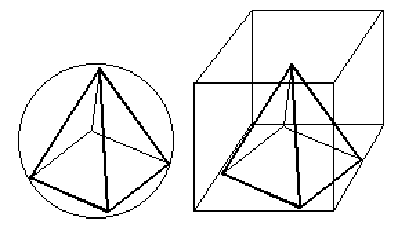
\includegraphics[width=0.6\textwidth]{img/shell.png}
		\caption{Сферическая и прямоугольная оболочки}}
\end{figure}

В дальнейшем при рассмотрении пересечения луча и объемной оболочкой рассматриваемого объекта, если такого пересечения нет, то и соответственно пересечения луча и самого рассматриваемого объекта нет, и наоборот, если мы найдем пересечение, то возможно, есть пересечение луча и рассматриваемого объекта. Для расчета эффектов освещения сцены проводятся вторичные лучи от точек пересечения ко всем источникам света. Если на пути этих лучей встречается непрозрачное тело, значит данная точка находится в тени, иначе он влияет на освещение данной точки. Также для получения более реалистичного изображения сцены, нужно учитывать вклады отраженных и преломленных лучей. 

К недостатку алгоритма относится его производительность. 
%Положительной стороной данного алгоритма является возможность использования в параллельных вычислительных системах (т.к. расчет отдельной точки выполняется независимо от других точек).

\section {Модель освещения}

Для создания реалистичного изображения в компьютерной графике применяются различные алгоритмы освещения.

Модель освещения предназначена для расчёта интенсивности
отражённого к наблюдателю света в каждой точке изображения.

Модель освещения может быть глобальной или локальной.

Локальная модель - учитывается только свет от источников и ориентация поверхности.

Локальная модель включает 3 составляющих: 

\begin{enumerate}
	\item Диффузную составляющую отражения.
	\item Отражающую составляющую отражения.
	\item Рассеянное освещение.
\end{enumerate}

Глобальная модель - учитывается ещё и свет, отражённый от других поверхностей или пропущенный через них

Глобальная модель воспроизводит чрезвычайно важные эффекты, которые будут показаны в данном проекте.

%Таким образом, глобальная модель освещения является частью алгоритмов выделения видимых поверхностей путём трассировки лучей.

\section {Преобразования}

\subsection {Некоторые теоретические сведения}

Преобразования на плоскости - изменение значений точек на плоскости:

\begin{equation}
A(x,y)\rightarrow B(x_1,y_1)
\end{equation}

Линейное преобразование:

\begin{equation}
{\begin{cases} 
	x_1 = Ax + By + C  \\
	y_1 = Dx + Ey + F  \\
	\end{cases}}
\end{equation}

Однородные координаты:

\begin{equation}
(x, y, w)
\end{equation}

Где w - масштабный множитель (для плоского случая w = 1), в обратном случае:

\begin{equation}
{\begin{cases} 
	x' = x / w  \\
	y' = y / w.  \\
	\end{cases}}
\end{equation}

Матрица преобразований:

\begin{equation}
Mtr = \left(
\begin{array}{cccc}
A & D & 0 \\
B & E & 0 \\
C & F & 1 \\
\end{array}
\right)
\end{equation}

Тогда, используя однородные координаты и матрицу преобразования, мы можем получить результат преобразования:

\begin{equation}
(x_1, y_1, 1) = (x, y, 1) * Mtr
\end{equation}

Методы двумерных преобразований распространяются и на изображения трехмерных объектов. Матрица преобразований  в трехмерном пространстве  в однородных координатах будет иметь размерность 4*4, а точки (x, y, z) заменяются четверткой (xw, yw, zw, w), w ≠ 0

\subsection {Перенос}

Для переноса нам потребуется два параметра: dx - смещение по оси абсцисс и dy - смещение по оси ординат.

\begin{equation}
{\begin{cases} 
	x_1 = x + dx  \\
	y_1 = y + dy  \\
	\end{cases}}
\end{equation}

Матрица переноса в двухмерном пространстве:

\begin{equation}
Mmove = \left(
\begin{array}{cccc}
1 & 0 & 0 \\
0 & 1 & 0 \\
dx & dy & 1 \\
\end{array}
\right)
\end{equation}

Матрица переноса в трехмерном пространстве:

\begin{equation}
Mmove = \left(
\begin{array}{cccc}
1 & 0 & 0 & 0 \\
0 & 1 & 0 & 0 \\
0 & 0 & 1 & 0 \\
dx & dy & dz & 1 \\
\end{array}
\right)
\end{equation}

\subsection {Масштабирование}

Масштабирование - изменение размера. Задается коэффициентами масштабирования kx, ky и центром масштабирования xm, ym. Иллюстрация представлена на рисунке \ref{fig:ref1} \\
\begin{figure}[ht!]
	\centering{
		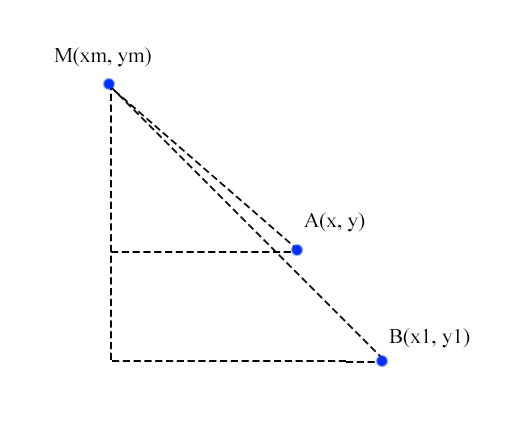
\includegraphics[width=0.6\textwidth]{img/move.jpg}
		\caption{Перемещение точки}
		\label{fig:ref1}}
\end{figure} 
\\
kx = ky - масштабирование однородное.\\
kx != ky - масштабирование неоднородное.\\
Отражение относительно OY: kx = -1, ky = 1.\\
Отражение относительно OX: kx = 1, ky = -1.\\
Отражение относительно начала координат: kx = -1, ky = -1.\\
Если коэффициент масштабирования больше 1, то изображение удаляется от центра и увеличивается.\\
Если коэффициент масштабирование меньше 1, то изображение приближается от центра и уменьшается.\\

Из Рис. \ref{fig:ref1} получаем:

\begin{equation}
{\begin{cases} 
	x_1 - x_m = kx(x - x_m)  \\
	y_1 - y_m = ky(y - y_m)  \\
	\label{eq:ref4}
	\end{cases}}
\end{equation}

Упростим (\ref{eq:ref4}) и получим: 

\begin{equation}
{\begin{cases} 
x_1 = kx * x + (1 - kx) * x_m \\
y_1 = ky * y + (1 - ky) * y_m \\
	\end{cases}}
\end{equation}

Матрица масштабирования в двухмерном пространстве:

\begin{equation}
Mscale = \left(
\begin{array}{cccc}
kx & 0 & 0 \\
0 & ky & 0 \\
0 & 0 & 1 \\
\end{array}
\right)
\end{equation}

Матрица масштабирования в трехмерном пространстве (Добавляется коэффициентами масштабирования: kz):

\begin{equation}
Mscale = \left(
\begin{array}{cccc}
kx & 0 & 0 & 0 \\
0 & ky & 0 & 0 \\
0 & 0 & kz & 0 \\
0 & 0 & 0 & 1 \\
\end{array}
\right)
\end{equation}

\subsection {Поворот}

Для поворота нам потребуется угол  $\theta$ и центр C(xc, yc).
\begin{figure}[ht!]
	\centering{
		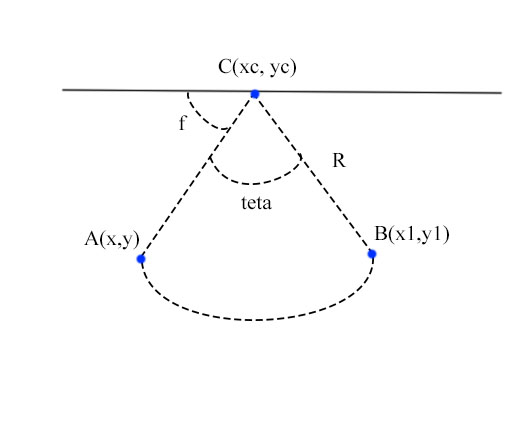
\includegraphics[width=0.6\textwidth]{img/rotate.jpg}
		\caption{Поворот точки}
		\label{fig:ref2}}
\end{figure} 

Вывод поворота против часовой стрелки:

\begin{multline}
\\
x_1 = x_c + R*cos(180^{\circ}-(\varphi +  \theta)) = \\
x_c - R*cos(\varphi)*cos(\theta) + R*sin(\varphi)*sin(\theta) = \\ 
x_c - (x_c - x)cos(\theta) + (y - y_c)sin(\theta) = \\ 
x_c + (x - x_c)cos(\theta) + (y - y_c)sin(\theta) \\
\end{multline}

\begin{multline}
\\
y_1 = y_c + R*sin(180^{\circ}-(\varphi +  \theta)) = \\
y_c + R*sin(\varphi)*cos(\theta) + R*cos(\varphi)*sin(\theta) = \\ 
y_c + (y - y_c)cos(\theta) + (x_c- x)sin(\theta) = \\ 
y_c + (y - y_c)cos(\theta) - (x - x_c)sin(\theta) \\
\end{multline}

Матрица поворота против часовой стрелки в двухмерном пространстве:

\begin{equation}
Mrotate = \left(
\begin{array}{cccc}
cos(\theta) & -sin(\theta) & 0 \\
sin(\theta) & cos(\theta) & 0 \\
0 & 0 & 1 \\
\end{array}
\right)
\end{equation}

Матрица поворота в трехмерном пространстве вокруг оси Z :

\begin{equation}
Mrotate = \left(
\begin{array}{cccc}
cos(\theta) & -sin(\theta) & 0 & 0 \\
sin(\theta) & cos(\theta) & 0 & 0 \\
0 & 0 & 1 & 0 \\
0 & 0 & 0 & 1 \\
\end{array}
\right)
\end{equation}

\section {Вывод}

Оценив все изложенные выше алгоритмы, можно сделать вывод, что для данной работы, которая предполагает визуализацию реалистического изображения, учитывая тени, отражение объектов и тд, подходит алгоритм обратной трассировки лучей, так как он позволяет достичь высокой реалистичности построенного изображения. Он будет использоваться, несмотря на указанные недостатки, так как алгоритм достаточно полно отражает суть физических явлений с приемлемыми затратами производительности.

% Так как недостатком алгоритма обратной трассировки лучей является низкая производительность, целесообразно подумать о ее улучшении, например, реализовать его многопоточное выполнение.